%%%%%%%%%%%%%%%%%%%%%%%%%%%%%%%%%%%%%%%%%%%%%%%%%%%%%%%%%%%%%%
\subsection{Детектирование ШПС от одного источника}
Рассмотрим простой случай - поиск гармонического сигнала на фоне АБГШ (интерференция отсутствует).

Пусть входной сигнал после снятия кода может быть представлен в виде:
\begin{center}
\begin{equation}
	\label{eq:lpc_signal_model1}
	x(k) = AC(k)D(k)\cos(\omega k + \phi(k)) + n(k)
\end{equation}
\end{center}
где: ${A}$ - мощность сигнала, ${C}$ - ПСП, ${D}$ - данные, а ${\omega_{c}}$ - частота несущей сигнала.
Детектирование сигнала происходит в пределах одного бита данных. В этом случае ${D(k)}$
принимается как константа. Повторная модуляция сигнала приводит к выражению ${C(k)C(k)=1}$.
Таким образом \ref{eq:lpc_signal_model1} можно записать как:
\begin{center}
\begin{equation}
	\label{eq:lpc_signal_model2}
	x(k)= A \cos{(\omega k)} + z(k)
\end{equation}
\end{center}

Поскольку ${n(k)}$ - случайный процесс, то ${z(k) = n(k)C(k)}$ также является
случайным процессом. Определим числовые характеристики ${z(k)}$.
В виду того что ${C(k)}$ и ${n(k)}$ - независимы, а ${D[C] = 1}$,можно записать:
\begin{center}
\begin{equation}
	%\label{}
	D[z(k)] = D[nC] = D[n] = \sigma ^2
\end{equation}
\end{center}
Таким образом ${z(k)}$ - АБГШ помеха.

Для уравнения \ref{eq:lpc_signal_model1}, необходимо вычислить ковариации для 3 точек
${r_{xx}(0)}$, ${r_{xx}(1)}$, ${r_{xx}(2)}$, используя выражение \ref{eq:lpc_rxx_estimation}.
Оценка частоты сигнала может быть получена из выражения \ref{eq:lpc_poles_freq}, а его
мощность из \ref{eq:lpc_power_cos}.

Можно построить график оценки СПМ для смещения,
содержащего максимальный спектральный пик - гармоническую компоненту
с наивысшей энергией - рисунок \ref{pic:lpc_psd_1} и график состоящий из максимальных спектральных пиков для каждой фазы
ПСП - рисунок \ref{pic:lpc_1sat_energy}.

\begin{figure}[H]
	\center\scalebox{1}{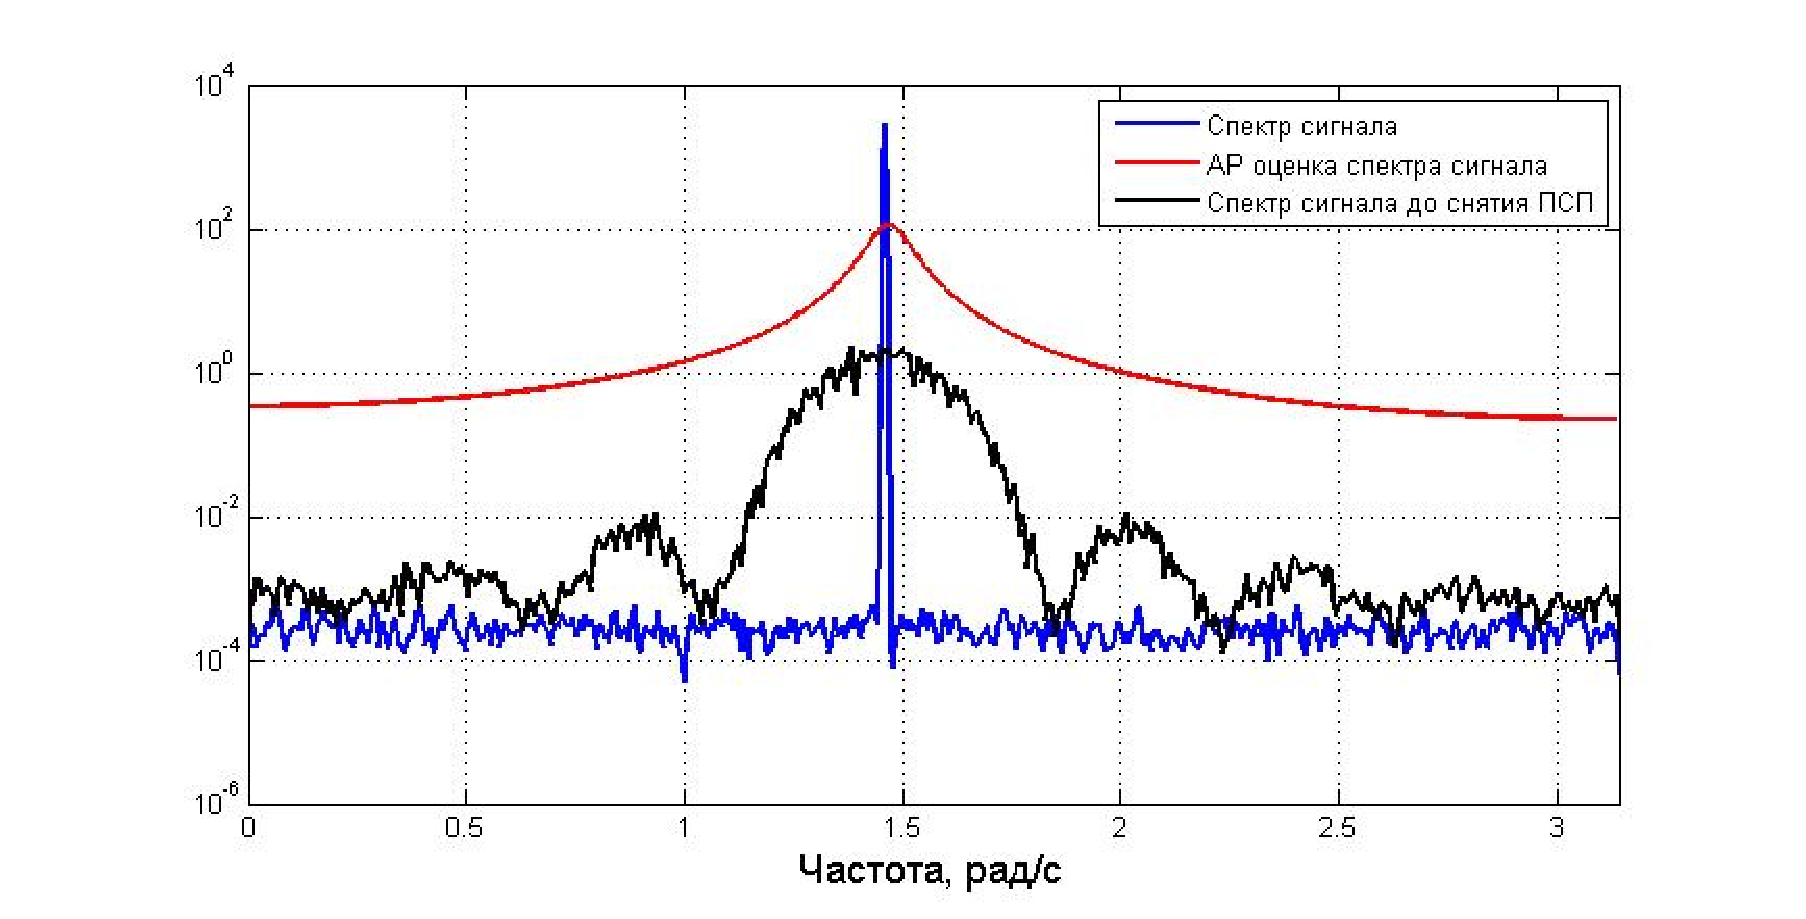
\includegraphics[width=1\linewidth]{lpc_1sat.eps}}
	\caption{Оценка СПМ сигнала модулированного ПСП}
	\label{pic:lpc_psd_1}
\end{figure}
\begin{figure}[H]
	\center\scalebox{1}{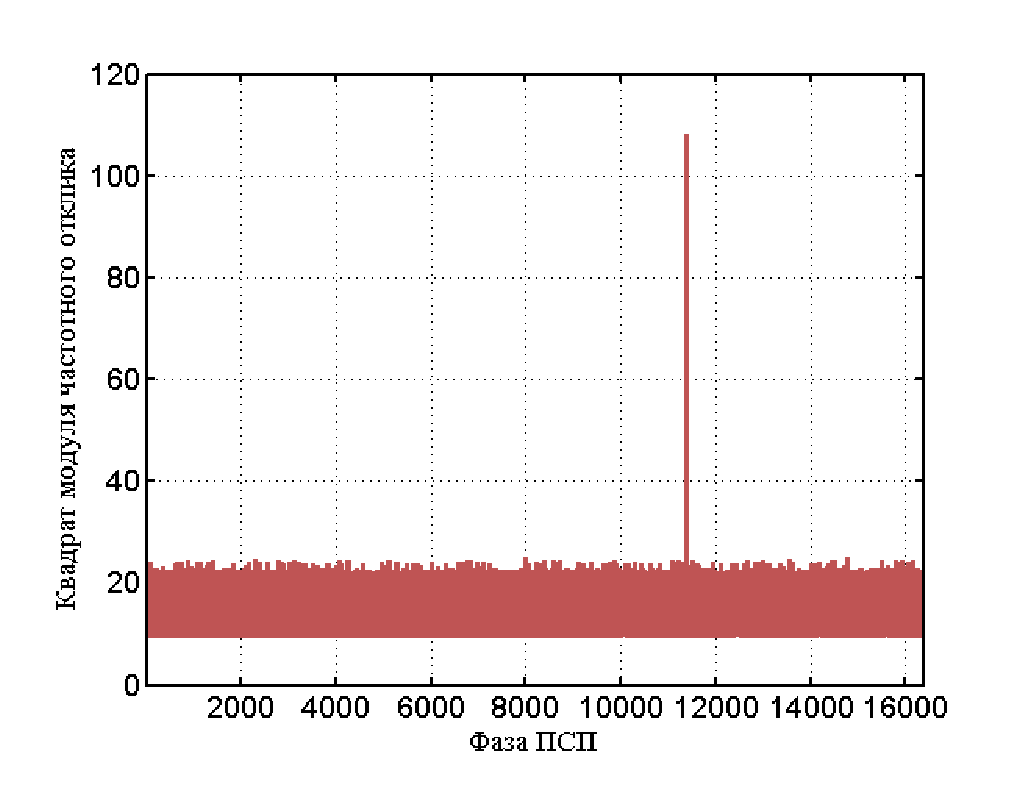
\includegraphics[width=1\linewidth]{lpc_1sat_energy.eps}}
	\caption{Квадраты частотного отклика для всех возможных фаз ПСП}
	\label{pic:lpc_1sat_energy}
\end{figure}



%%%%%%%%%%%%%%%%%%%%%%%%%%%%%%%%%%%%%%%%%%%%%%%%%%%%%%%%%%%%%%
\subsubsection{Влияние интерференции на точность детектирования с помощью АР модели}
Шум, отличный АБГШ будет смещать оценку частоты. На рисунке \ref{pic:lpc_2sat_psd} показано
смещение для интерференционной помехи от еще одного источника сигнала, модулированной ПСП того же семейства.
Данная помеха не является белой и оценка АР-методом по предложенному алгоритму не даст надежной оценки частоты сигнала.

\begin{figure}[H]
	\center\scalebox{1}{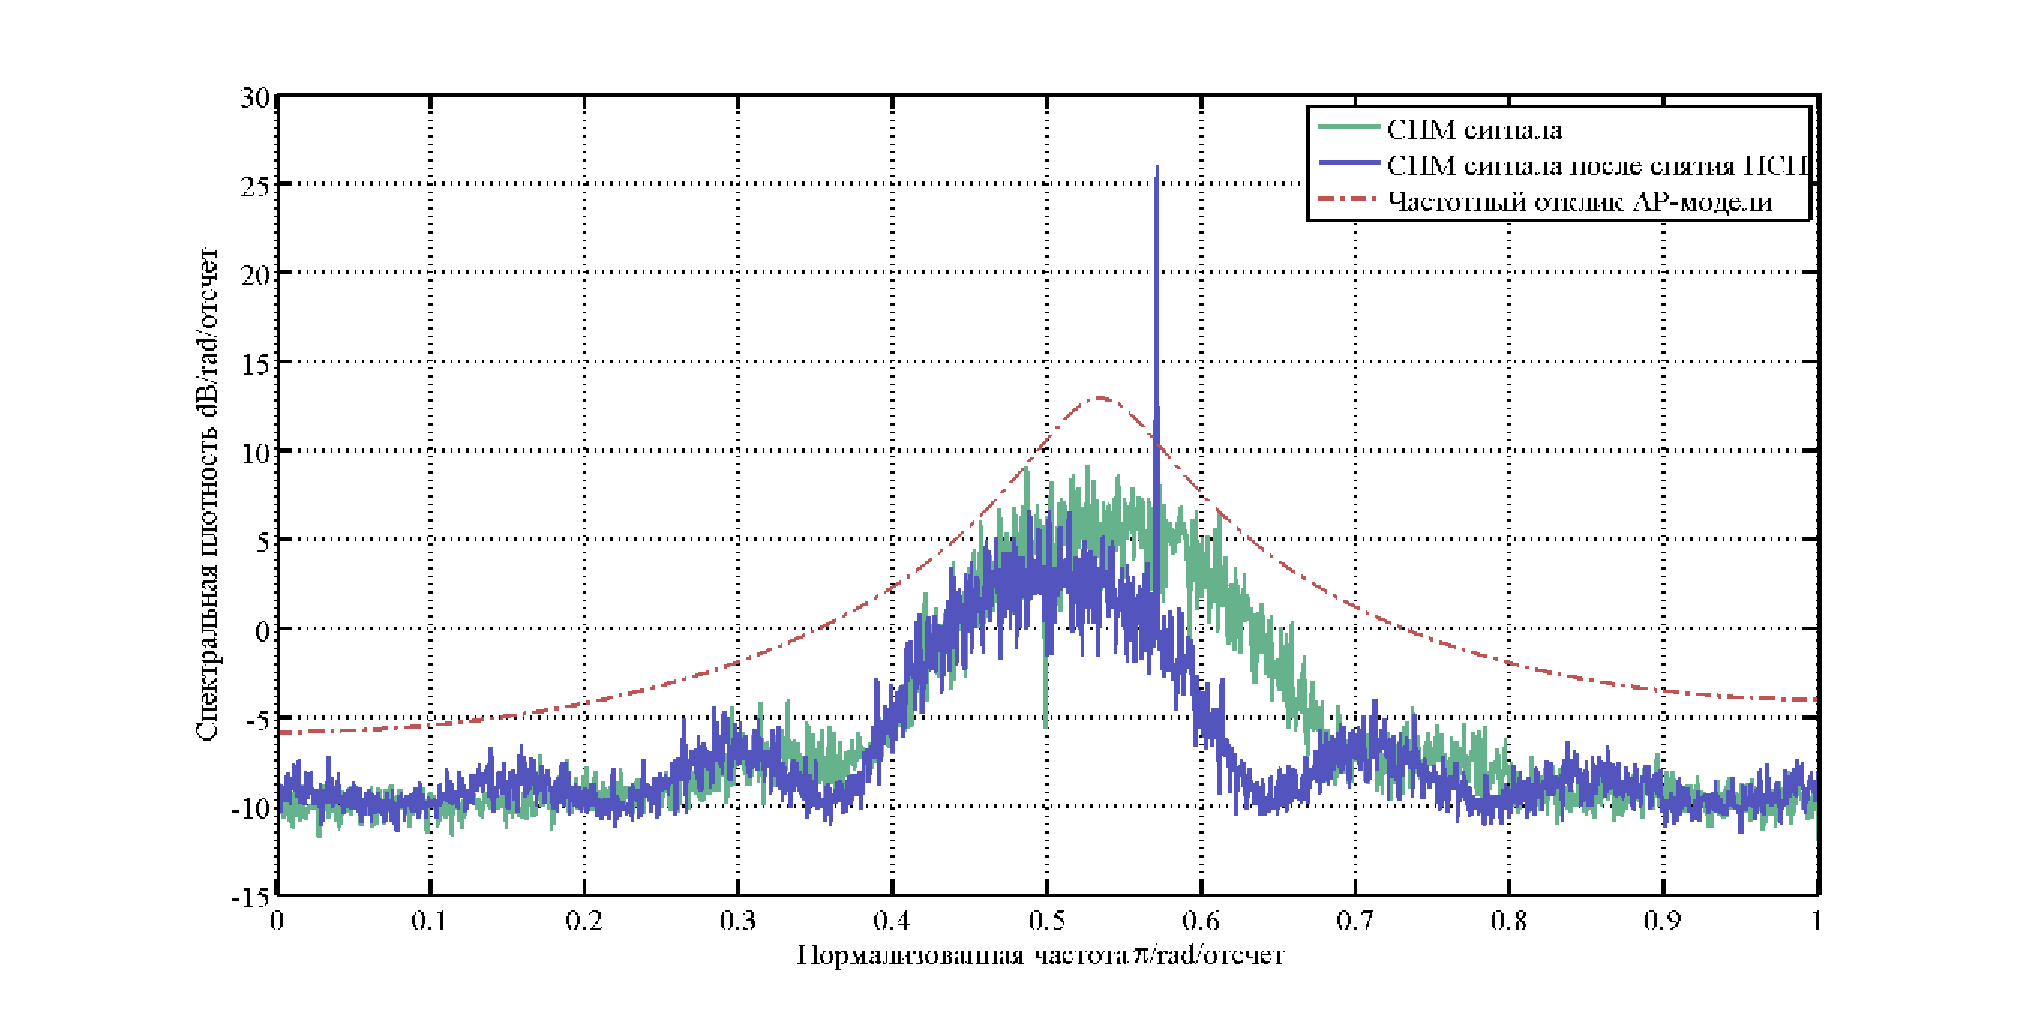
\includegraphics[width=1\linewidth]{lpc_2sat_psd.eps}}
	\caption{СПМ для сигнала с интерференционной помехой}
	\label{pic:lpc_2sat_psd}
\end{figure}

\subsection*{Выводы}
\label{ssec:sec3_lpc_conclusion}

В данном разделе предложен алгоритм детектирования ШПС на основе АР-модели принимаемого сигнала.
Разработанный алгоритм позволяет производить оценку частоты гармонического сигнала без использования прямого
перебора как это делается в большинстве современных алгоритмов. Например, алгоритм Delay and Multiply Approach (DMA) предложенный в 
\cite{lin_dma, tsui} позволяет производить поиск только по смещению ПСП, но он не дает возможности прямой оценки частоты.
Для оценки частоты и принятия решения о наличии сигнала в алгоритме DMA необходимо использовать стандартный коррелятор.

К недостаткам данного подхода можно отнести: 
\begin{enumerate}
	\item Сравнительно высокие вычислительные затраты. Предложенный алгоритм требует поиск гармонической
		компоненты, а так же обращения теплицевой матрицы для каждого смещения ПСП.
	\item Сильная чувствительность по отношению к интерференционным помехам: наличие
		''окрашенного'' шума приводит к значительному смещению получаемых
		оценок частоты и мощности гармонического сигнала.
\end{enumerate}
